\documentclass[11pt]{article}
\newcommand{\LabNumber}{2}
\newcommand{\LabTitle}{The EC-1 Microprocessor}
\newcommand{\LabTopic}{ISA, datapath construction, and hardwired FSM control-unit design in Logisim-Evolution}
% Shared preamble for Computer Programming lab sheets.
% Include with % Shared preamble for Computer Programming lab sheets.
% Include with % Shared preamble for Computer Programming lab sheets.
% Include with \input{common.tex} after \documentclass{article}.

\usepackage[a4paper,margin=2.2cm]{geometry}
\usepackage[T1]{fontenc}
\usepackage{lmodern}
\usepackage{microtype}
\usepackage{enumitem}
\usepackage{xcolor}
\usepackage{tcolorbox}
\tcbuselibrary{breakable,skins}
\usepackage{listings}
\usepackage{fancyhdr}
\usepackage{titlesec}
\usepackage{amsmath}
\usepackage{array}
\usepackage{booktabs}
\usepackage{hyperref}

\hypersetup{
  colorlinks=true,
  linkcolor=black,
  urlcolor=blue!60!black,
  pdfborder={0 0 0}
}

% ---------- Course identity (override per file if needed) ----------
\providecommand{\CourseName}{Microprocessors}
\providecommand{\CourseCode}{010153521}
\providecommand{\Semester}{Semester 1/2026}
\providecommand{\LabDuration}{3 hours (in-lab)}

% ---------- Colors ----------
\definecolor{accent}{HTML}{1F4E79}
\definecolor{accentlight}{HTML}{D9E2EC}
\definecolor{warn}{HTML}{B45309}
\definecolor{ok}{HTML}{166534}
\definecolor{codebg}{HTML}{F6F8FA}
\definecolor{codeframe}{HTML}{D0D7DE}
\definecolor{codekw}{HTML}{0550AE}
\definecolor{codestr}{HTML}{0A7B2C}
\definecolor{codecom}{HTML}{6E7781}

% ---------- Code / assembly listings ----------
\lstdefinestyle{c}{
  language=C,
  basicstyle=\ttfamily\small,
  keywordstyle=\color{codekw}\bfseries,
  stringstyle=\color{codestr},
  commentstyle=\color{codecom}\itshape,
  backgroundcolor=\color{codebg},
  frame=single,
  rulecolor=\color{codeframe},
  framerule=0.4pt,
  showstringspaces=false,
  breaklines=true,
  columns=fullflexible,
  keepspaces=true,
  tabsize=4,
  xleftmargin=8pt,
  xrightmargin=4pt,
  aboveskip=6pt,
  belowskip=6pt,
}
\lstdefinestyle{asm}{
  basicstyle=\ttfamily\small,
  commentstyle=\color{codecom}\itshape,
  backgroundcolor=\color{codebg},
  frame=single,
  rulecolor=\color{codeframe},
  framerule=0.4pt,
  showstringspaces=false,
  breaklines=true,
  columns=fullflexible,
  keepspaces=true,
  tabsize=4,
  xleftmargin=8pt,
  xrightmargin=4pt,
  aboveskip=6pt,
  belowskip=6pt,
}
\lstset{style=asm}

% ---------- Section styling ----------
\titleformat{\section}{\Large\bfseries\color{accent}}{\thesection.}{0.5em}{}
\titleformat{\subsection}{\large\bfseries\color{accent!85!black}}{\thesubsection}{0.5em}{}
\titlespacing*{\section}{0pt}{12pt}{6pt}
\titlespacing*{\subsection}{0pt}{8pt}{4pt}

% ---------- Page headers/footers ----------
\pagestyle{fancy}
\fancyhf{}
\fancyhead[L]{\small\CourseName\ifx\CourseCode\empty\else\ (\CourseCode)\fi}
\fancyhead[C]{\small\Semester}
\fancyhead[R]{\small\textbf{Lab \LabNumber:} \LabTitle}
\fancyfoot[C]{\small\thepage}
\renewcommand{\headrulewidth}{0.4pt}

% ---------- Title block ----------
\newcommand{\labheader}{%
  \begin{tcolorbox}[
    enhanced,
    colback=accentlight,
    colframe=accent,
    boxrule=0.5pt,
    arc=2pt,
    left=10pt, right=10pt, top=8pt, bottom=8pt
  ]
    {\Large\bfseries\color{accent} Lab \LabNumber: \LabTitle}\\[2pt]
    {\small \CourseName\ifx\CourseCode\empty\else\ (\CourseCode)\fi\quad\textbar\quad \Semester}\\[1pt]
    {\small \textbf{Duration:} \LabDuration\quad\textbar\quad \textbf{Topic:} \LabTopic}
  \end{tcolorbox}
  \vspace{2pt}
}

% ---------- Custom environments ----------
\newtcolorbox{summary}[1][Quick Reference]{
  enhanced,breakable,
  colback=accentlight!40,colframe=accent!70,
  title={\bfseries #1},
  fonttitle=\color{white},
  attach boxed title to top left={xshift=6pt,yshift=-3pt},
  boxed title style={colback=accent,boxrule=0pt,arc=2pt},
  arc=2pt,boxrule=0.4pt,
  top=12pt,
}

\newcounter{labex}[section]
\newtcolorbox{labexercise}[1]{
  enhanced,breakable,
  colback=white,colframe=accent,
  title={\bfseries In-Lab Exercise \refstepcounter{labex}\thelabex: #1},
  fonttitle=\color{white},
  attach boxed title to top left={xshift=6pt,yshift=-3pt},
  boxed title style={colback=accent,boxrule=0pt,arc=2pt},
  arc=2pt,boxrule=0.4pt,
  top=12pt,
}

\newcounter{traceex}
\newtcolorbox{trace}[1][]{
  enhanced,breakable,
  colback=white,colframe=warn,
  title={\bfseries Trace \& Predict \refstepcounter{traceex}\thetraceex\ifx\\#1\\\else: #1\fi},
  fonttitle=\color{white},
  attach boxed title to top left={xshift=6pt,yshift=-3pt},
  boxed title style={colback=warn,boxrule=0pt,arc=2pt},
  arc=2pt,boxrule=0.4pt,
  top=12pt,
}

\newcounter{bugex}
\newtcolorbox{bug}[1][]{
  enhanced,breakable,
  colback=white,colframe=warn,
  title={\bfseries Find the Bug \refstepcounter{bugex}\thebugex\ifx\\#1\\\else: #1\fi},
  fonttitle=\color{white},
  attach boxed title to top left={xshift=6pt,yshift=-3pt},
  boxed title style={colback=warn,boxrule=0pt,arc=2pt},
  arc=2pt,boxrule=0.4pt,
  top=12pt,
}

\newcounter{writeex}
\newtcolorbox{writecode}[1][]{
  enhanced,breakable,
  colback=white,colframe=warn,
  title={\bfseries Write Code on Paper \refstepcounter{writeex}\thewriteex\ifx\\#1\\\else: #1\fi},
  fonttitle=\color{white},
  attach boxed title to top left={xshift=6pt,yshift=-3pt},
  boxed title style={colback=warn,boxrule=0pt,arc=2pt},
  arc=2pt,boxrule=0.4pt,
  top=12pt,
}

% ---------- AI Collaboration box ----------
\definecolor{aipurple}{HTML}{4C1D95}
\definecolor{aipurplelight}{HTML}{EDE9FE}

\newtcolorbox{aicollab}[1][AI Collaboration]{
  enhanced,breakable,
  colback=aipurplelight,colframe=aipurple!70,
  title={\bfseries #1},
  fonttitle=\color{white},
  attach boxed title to top left={xshift=6pt,yshift=-3pt},
  boxed title style={colback=aipurple,boxrule=0pt,arc=2pt},
  arc=2pt,boxrule=0.4pt,
  top=12pt,
}

\newcounter{tryex}
\newtcolorbox{tryit}[1]{
  enhanced,breakable,
  colback=ok!6,colframe=ok!70!black,
  title={\bfseries Try It \refstepcounter{tryex}\thetryex: #1},
  fonttitle=\color{white},
  attach boxed title to top left={xshift=6pt,yshift=-3pt},
  boxed title style={colback=ok!70!black,boxrule=0pt,arc=2pt},
  arc=2pt,boxrule=0.4pt,
  top=12pt,
}

% ---------- Drawing exercise ----------
\definecolor{drawteal}{HTML}{0D7377}
\definecolor{drawteallight}{HTML}{D4F1F4}

\newcounter{drawex}
\newtcolorbox{drawex}[1]{
  enhanced,breakable,
  colback=drawteallight,colframe=drawteal!70,
  title={\bfseries Draw on Paper \refstepcounter{drawex}\thedrawex: #1},
  fonttitle=\color{white},
  attach boxed title to top left={xshift=6pt,yshift=-3pt},
  boxed title style={colback=drawteal,boxrule=0pt,arc=2pt},
  arc=2pt,boxrule=0.4pt,
  top=12pt,
}


\newcommand{\takehomebanner}{%
  \vspace{6pt}
  \begin{tcolorbox}[
    colback=warn!10,colframe=warn,boxrule=0.5pt,arc=2pt,
    left=10pt,right=10pt,top=6pt,bottom=6pt
  ]
    \textbf{Take-Home (Paper Work).}\;
    Solve the following on paper without using a computer or compiler.
    Hand-write your answers; submit at the start of the next lab.
    Goal: prepare you to dry-code during the written exam.
  \end{tcolorbox}
  \vspace{4pt}
}
 after \documentclass{article}.

\usepackage[a4paper,margin=2.2cm]{geometry}
\usepackage[T1]{fontenc}
\usepackage{lmodern}
\usepackage{microtype}
\usepackage{enumitem}
\usepackage{xcolor}
\usepackage{tcolorbox}
\tcbuselibrary{breakable,skins}
\usepackage{listings}
\usepackage{fancyhdr}
\usepackage{titlesec}
\usepackage{amsmath}
\usepackage{array}
\usepackage{booktabs}
\usepackage{hyperref}

\hypersetup{
  colorlinks=true,
  linkcolor=black,
  urlcolor=blue!60!black,
  pdfborder={0 0 0}
}

% ---------- Course identity (override per file if needed) ----------
\providecommand{\CourseName}{Microprocessors}
\providecommand{\CourseCode}{010153521}
\providecommand{\Semester}{Semester 1/2026}
\providecommand{\LabDuration}{3 hours (in-lab)}

% ---------- Colors ----------
\definecolor{accent}{HTML}{1F4E79}
\definecolor{accentlight}{HTML}{D9E2EC}
\definecolor{warn}{HTML}{B45309}
\definecolor{ok}{HTML}{166534}
\definecolor{codebg}{HTML}{F6F8FA}
\definecolor{codeframe}{HTML}{D0D7DE}
\definecolor{codekw}{HTML}{0550AE}
\definecolor{codestr}{HTML}{0A7B2C}
\definecolor{codecom}{HTML}{6E7781}

% ---------- Code / assembly listings ----------
\lstdefinestyle{c}{
  language=C,
  basicstyle=\ttfamily\small,
  keywordstyle=\color{codekw}\bfseries,
  stringstyle=\color{codestr},
  commentstyle=\color{codecom}\itshape,
  backgroundcolor=\color{codebg},
  frame=single,
  rulecolor=\color{codeframe},
  framerule=0.4pt,
  showstringspaces=false,
  breaklines=true,
  columns=fullflexible,
  keepspaces=true,
  tabsize=4,
  xleftmargin=8pt,
  xrightmargin=4pt,
  aboveskip=6pt,
  belowskip=6pt,
}
\lstdefinestyle{asm}{
  basicstyle=\ttfamily\small,
  commentstyle=\color{codecom}\itshape,
  backgroundcolor=\color{codebg},
  frame=single,
  rulecolor=\color{codeframe},
  framerule=0.4pt,
  showstringspaces=false,
  breaklines=true,
  columns=fullflexible,
  keepspaces=true,
  tabsize=4,
  xleftmargin=8pt,
  xrightmargin=4pt,
  aboveskip=6pt,
  belowskip=6pt,
}
\lstset{style=asm}

% ---------- Section styling ----------
\titleformat{\section}{\Large\bfseries\color{accent}}{\thesection.}{0.5em}{}
\titleformat{\subsection}{\large\bfseries\color{accent!85!black}}{\thesubsection}{0.5em}{}
\titlespacing*{\section}{0pt}{12pt}{6pt}
\titlespacing*{\subsection}{0pt}{8pt}{4pt}

% ---------- Page headers/footers ----------
\pagestyle{fancy}
\fancyhf{}
\fancyhead[L]{\small\CourseName\ifx\CourseCode\empty\else\ (\CourseCode)\fi}
\fancyhead[C]{\small\Semester}
\fancyhead[R]{\small\textbf{Lab \LabNumber:} \LabTitle}
\fancyfoot[C]{\small\thepage}
\renewcommand{\headrulewidth}{0.4pt}

% ---------- Title block ----------
\newcommand{\labheader}{%
  \begin{tcolorbox}[
    enhanced,
    colback=accentlight,
    colframe=accent,
    boxrule=0.5pt,
    arc=2pt,
    left=10pt, right=10pt, top=8pt, bottom=8pt
  ]
    {\Large\bfseries\color{accent} Lab \LabNumber: \LabTitle}\\[2pt]
    {\small \CourseName\ifx\CourseCode\empty\else\ (\CourseCode)\fi\quad\textbar\quad \Semester}\\[1pt]
    {\small \textbf{Duration:} \LabDuration\quad\textbar\quad \textbf{Topic:} \LabTopic}
  \end{tcolorbox}
  \vspace{2pt}
}

% ---------- Custom environments ----------
\newtcolorbox{summary}[1][Quick Reference]{
  enhanced,breakable,
  colback=accentlight!40,colframe=accent!70,
  title={\bfseries #1},
  fonttitle=\color{white},
  attach boxed title to top left={xshift=6pt,yshift=-3pt},
  boxed title style={colback=accent,boxrule=0pt,arc=2pt},
  arc=2pt,boxrule=0.4pt,
  top=12pt,
}

\newcounter{labex}[section]
\newtcolorbox{labexercise}[1]{
  enhanced,breakable,
  colback=white,colframe=accent,
  title={\bfseries In-Lab Exercise \refstepcounter{labex}\thelabex: #1},
  fonttitle=\color{white},
  attach boxed title to top left={xshift=6pt,yshift=-3pt},
  boxed title style={colback=accent,boxrule=0pt,arc=2pt},
  arc=2pt,boxrule=0.4pt,
  top=12pt,
}

\newcounter{traceex}
\newtcolorbox{trace}[1][]{
  enhanced,breakable,
  colback=white,colframe=warn,
  title={\bfseries Trace \& Predict \refstepcounter{traceex}\thetraceex\ifx\\#1\\\else: #1\fi},
  fonttitle=\color{white},
  attach boxed title to top left={xshift=6pt,yshift=-3pt},
  boxed title style={colback=warn,boxrule=0pt,arc=2pt},
  arc=2pt,boxrule=0.4pt,
  top=12pt,
}

\newcounter{bugex}
\newtcolorbox{bug}[1][]{
  enhanced,breakable,
  colback=white,colframe=warn,
  title={\bfseries Find the Bug \refstepcounter{bugex}\thebugex\ifx\\#1\\\else: #1\fi},
  fonttitle=\color{white},
  attach boxed title to top left={xshift=6pt,yshift=-3pt},
  boxed title style={colback=warn,boxrule=0pt,arc=2pt},
  arc=2pt,boxrule=0.4pt,
  top=12pt,
}

\newcounter{writeex}
\newtcolorbox{writecode}[1][]{
  enhanced,breakable,
  colback=white,colframe=warn,
  title={\bfseries Write Code on Paper \refstepcounter{writeex}\thewriteex\ifx\\#1\\\else: #1\fi},
  fonttitle=\color{white},
  attach boxed title to top left={xshift=6pt,yshift=-3pt},
  boxed title style={colback=warn,boxrule=0pt,arc=2pt},
  arc=2pt,boxrule=0.4pt,
  top=12pt,
}

% ---------- AI Collaboration box ----------
\definecolor{aipurple}{HTML}{4C1D95}
\definecolor{aipurplelight}{HTML}{EDE9FE}

\newtcolorbox{aicollab}[1][AI Collaboration]{
  enhanced,breakable,
  colback=aipurplelight,colframe=aipurple!70,
  title={\bfseries #1},
  fonttitle=\color{white},
  attach boxed title to top left={xshift=6pt,yshift=-3pt},
  boxed title style={colback=aipurple,boxrule=0pt,arc=2pt},
  arc=2pt,boxrule=0.4pt,
  top=12pt,
}

\newcounter{tryex}
\newtcolorbox{tryit}[1]{
  enhanced,breakable,
  colback=ok!6,colframe=ok!70!black,
  title={\bfseries Try It \refstepcounter{tryex}\thetryex: #1},
  fonttitle=\color{white},
  attach boxed title to top left={xshift=6pt,yshift=-3pt},
  boxed title style={colback=ok!70!black,boxrule=0pt,arc=2pt},
  arc=2pt,boxrule=0.4pt,
  top=12pt,
}

% ---------- Drawing exercise ----------
\definecolor{drawteal}{HTML}{0D7377}
\definecolor{drawteallight}{HTML}{D4F1F4}

\newcounter{drawex}
\newtcolorbox{drawex}[1]{
  enhanced,breakable,
  colback=drawteallight,colframe=drawteal!70,
  title={\bfseries Draw on Paper \refstepcounter{drawex}\thedrawex: #1},
  fonttitle=\color{white},
  attach boxed title to top left={xshift=6pt,yshift=-3pt},
  boxed title style={colback=drawteal,boxrule=0pt,arc=2pt},
  arc=2pt,boxrule=0.4pt,
  top=12pt,
}


\newcommand{\takehomebanner}{%
  \vspace{6pt}
  \begin{tcolorbox}[
    colback=warn!10,colframe=warn,boxrule=0.5pt,arc=2pt,
    left=10pt,right=10pt,top=6pt,bottom=6pt
  ]
    \textbf{Take-Home (Paper Work).}\;
    Solve the following on paper without using a computer or compiler.
    Hand-write your answers; submit at the start of the next lab.
    Goal: prepare you to dry-code during the written exam.
  \end{tcolorbox}
  \vspace{4pt}
}
 after \documentclass{article}.

\usepackage[a4paper,margin=2.2cm]{geometry}
\usepackage[T1]{fontenc}
\usepackage{lmodern}
\usepackage{microtype}
\usepackage{enumitem}
\usepackage{xcolor}
\usepackage{tcolorbox}
\tcbuselibrary{breakable,skins}
\usepackage{listings}
\usepackage{fancyhdr}
\usepackage{titlesec}
\usepackage{amsmath}
\usepackage{array}
\usepackage{booktabs}
\usepackage{hyperref}

\hypersetup{
  colorlinks=true,
  linkcolor=black,
  urlcolor=blue!60!black,
  pdfborder={0 0 0}
}

% ---------- Course identity (override per file if needed) ----------
\providecommand{\CourseName}{Microprocessors}
\providecommand{\CourseCode}{010153521}
\providecommand{\Semester}{Semester 1/2026}
\providecommand{\LabDuration}{3 hours (in-lab)}

% ---------- Colors ----------
\definecolor{accent}{HTML}{1F4E79}
\definecolor{accentlight}{HTML}{D9E2EC}
\definecolor{warn}{HTML}{B45309}
\definecolor{ok}{HTML}{166534}
\definecolor{codebg}{HTML}{F6F8FA}
\definecolor{codeframe}{HTML}{D0D7DE}
\definecolor{codekw}{HTML}{0550AE}
\definecolor{codestr}{HTML}{0A7B2C}
\definecolor{codecom}{HTML}{6E7781}

% ---------- Code / assembly listings ----------
\lstdefinestyle{c}{
  language=C,
  basicstyle=\ttfamily\small,
  keywordstyle=\color{codekw}\bfseries,
  stringstyle=\color{codestr},
  commentstyle=\color{codecom}\itshape,
  backgroundcolor=\color{codebg},
  frame=single,
  rulecolor=\color{codeframe},
  framerule=0.4pt,
  showstringspaces=false,
  breaklines=true,
  columns=fullflexible,
  keepspaces=true,
  tabsize=4,
  xleftmargin=8pt,
  xrightmargin=4pt,
  aboveskip=6pt,
  belowskip=6pt,
}
\lstdefinestyle{asm}{
  basicstyle=\ttfamily\small,
  commentstyle=\color{codecom}\itshape,
  backgroundcolor=\color{codebg},
  frame=single,
  rulecolor=\color{codeframe},
  framerule=0.4pt,
  showstringspaces=false,
  breaklines=true,
  columns=fullflexible,
  keepspaces=true,
  tabsize=4,
  xleftmargin=8pt,
  xrightmargin=4pt,
  aboveskip=6pt,
  belowskip=6pt,
}
\lstset{style=asm}

% ---------- Section styling ----------
\titleformat{\section}{\Large\bfseries\color{accent}}{\thesection.}{0.5em}{}
\titleformat{\subsection}{\large\bfseries\color{accent!85!black}}{\thesubsection}{0.5em}{}
\titlespacing*{\section}{0pt}{12pt}{6pt}
\titlespacing*{\subsection}{0pt}{8pt}{4pt}

% ---------- Page headers/footers ----------
\pagestyle{fancy}
\fancyhf{}
\fancyhead[L]{\small\CourseName\ifx\CourseCode\empty\else\ (\CourseCode)\fi}
\fancyhead[C]{\small\Semester}
\fancyhead[R]{\small\textbf{Lab \LabNumber:} \LabTitle}
\fancyfoot[C]{\small\thepage}
\renewcommand{\headrulewidth}{0.4pt}

% ---------- Title block ----------
\newcommand{\labheader}{%
  \begin{tcolorbox}[
    enhanced,
    colback=accentlight,
    colframe=accent,
    boxrule=0.5pt,
    arc=2pt,
    left=10pt, right=10pt, top=8pt, bottom=8pt
  ]
    {\Large\bfseries\color{accent} Lab \LabNumber: \LabTitle}\\[2pt]
    {\small \CourseName\ifx\CourseCode\empty\else\ (\CourseCode)\fi\quad\textbar\quad \Semester}\\[1pt]
    {\small \textbf{Duration:} \LabDuration\quad\textbar\quad \textbf{Topic:} \LabTopic}
  \end{tcolorbox}
  \vspace{2pt}
}

% ---------- Custom environments ----------
\newtcolorbox{summary}[1][Quick Reference]{
  enhanced,breakable,
  colback=accentlight!40,colframe=accent!70,
  title={\bfseries #1},
  fonttitle=\color{white},
  attach boxed title to top left={xshift=6pt,yshift=-3pt},
  boxed title style={colback=accent,boxrule=0pt,arc=2pt},
  arc=2pt,boxrule=0.4pt,
  top=12pt,
}

\newcounter{labex}[section]
\newtcolorbox{labexercise}[1]{
  enhanced,breakable,
  colback=white,colframe=accent,
  title={\bfseries In-Lab Exercise \refstepcounter{labex}\thelabex: #1},
  fonttitle=\color{white},
  attach boxed title to top left={xshift=6pt,yshift=-3pt},
  boxed title style={colback=accent,boxrule=0pt,arc=2pt},
  arc=2pt,boxrule=0.4pt,
  top=12pt,
}

\newcounter{traceex}
\newtcolorbox{trace}[1][]{
  enhanced,breakable,
  colback=white,colframe=warn,
  title={\bfseries Trace \& Predict \refstepcounter{traceex}\thetraceex\ifx\\#1\\\else: #1\fi},
  fonttitle=\color{white},
  attach boxed title to top left={xshift=6pt,yshift=-3pt},
  boxed title style={colback=warn,boxrule=0pt,arc=2pt},
  arc=2pt,boxrule=0.4pt,
  top=12pt,
}

\newcounter{bugex}
\newtcolorbox{bug}[1][]{
  enhanced,breakable,
  colback=white,colframe=warn,
  title={\bfseries Find the Bug \refstepcounter{bugex}\thebugex\ifx\\#1\\\else: #1\fi},
  fonttitle=\color{white},
  attach boxed title to top left={xshift=6pt,yshift=-3pt},
  boxed title style={colback=warn,boxrule=0pt,arc=2pt},
  arc=2pt,boxrule=0.4pt,
  top=12pt,
}

\newcounter{writeex}
\newtcolorbox{writecode}[1][]{
  enhanced,breakable,
  colback=white,colframe=warn,
  title={\bfseries Write Code on Paper \refstepcounter{writeex}\thewriteex\ifx\\#1\\\else: #1\fi},
  fonttitle=\color{white},
  attach boxed title to top left={xshift=6pt,yshift=-3pt},
  boxed title style={colback=warn,boxrule=0pt,arc=2pt},
  arc=2pt,boxrule=0.4pt,
  top=12pt,
}

% ---------- AI Collaboration box ----------
\definecolor{aipurple}{HTML}{4C1D95}
\definecolor{aipurplelight}{HTML}{EDE9FE}

\newtcolorbox{aicollab}[1][AI Collaboration]{
  enhanced,breakable,
  colback=aipurplelight,colframe=aipurple!70,
  title={\bfseries #1},
  fonttitle=\color{white},
  attach boxed title to top left={xshift=6pt,yshift=-3pt},
  boxed title style={colback=aipurple,boxrule=0pt,arc=2pt},
  arc=2pt,boxrule=0.4pt,
  top=12pt,
}

\newcounter{tryex}
\newtcolorbox{tryit}[1]{
  enhanced,breakable,
  colback=ok!6,colframe=ok!70!black,
  title={\bfseries Try It \refstepcounter{tryex}\thetryex: #1},
  fonttitle=\color{white},
  attach boxed title to top left={xshift=6pt,yshift=-3pt},
  boxed title style={colback=ok!70!black,boxrule=0pt,arc=2pt},
  arc=2pt,boxrule=0.4pt,
  top=12pt,
}

% ---------- Drawing exercise ----------
\definecolor{drawteal}{HTML}{0D7377}
\definecolor{drawteallight}{HTML}{D4F1F4}

\newcounter{drawex}
\newtcolorbox{drawex}[1]{
  enhanced,breakable,
  colback=drawteallight,colframe=drawteal!70,
  title={\bfseries Draw on Paper \refstepcounter{drawex}\thedrawex: #1},
  fonttitle=\color{white},
  attach boxed title to top left={xshift=6pt,yshift=-3pt},
  boxed title style={colback=drawteal,boxrule=0pt,arc=2pt},
  arc=2pt,boxrule=0.4pt,
  top=12pt,
}


\newcommand{\takehomebanner}{%
  \vspace{6pt}
  \begin{tcolorbox}[
    colback=warn!10,colframe=warn,boxrule=0.5pt,arc=2pt,
    left=10pt,right=10pt,top=6pt,bottom=6pt
  ]
    \textbf{Take-Home (Paper Work).}\;
    Solve the following on paper without using a computer or compiler.
    Hand-write your answers; submit at the start of the next lab.
    Goal: prepare you to dry-code during the written exam.
  \end{tcolorbox}
  \vspace{4pt}
}

\usepackage{graphicx}
\usepackage{tikz}
\usetikzlibrary{automata,positioning}

\begin{document}
\labheader

\section*{Objectives}
\begin{itemize}[leftmargin=*,nosep]
  \item Translate a datapath block diagram (registers, incrementer/decrementer, muxes,
        tri-state buffer) into working Logisim-Evolution components.
  \item Design a hardwired FSM control unit from an ISA and the fetch/decode/execute
        instruction cycle: choose states, draw the state diagram, encode it, and derive
        Boolean next-state and output equations.
  \item Hand-assemble an EC-1 program, load it into ROM, and verify its execution cycle
        by cycle.
\end{itemize}

\begin{summary}[Quick Reference: EC-1 ISA]
EC-1 is an 8-bit-data, 4-bit-address machine: 16 ROM locations, each holding one
8-bit instruction word (\texttt{IR[7:5]} = opcode, \texttt{IR[4:0]} = operand).
\begin{center}
\begin{tabular}{@{}llll@{}}
\toprule
\textbf{Instruction} & \textbf{Mnemonic} & \textbf{Encoding} & \textbf{Operation} \\
\midrule
Input        & \texttt{IN A}    & \texttt{011 xxxxx} & $A \leftarrow \text{Input}$ \\
Output       & \texttt{OUT A}   & \texttt{100 xxxxx} & $\text{Output} \leftarrow A$ \\
Decrement    & \texttt{DEC A}   & \texttt{101 xxxxx} & $A \leftarrow A - 1$ \\
Jump if Not Zero & \texttt{JNZ addr} & \texttt{110 xaaaa} & if $A \neq 0$: $PC \leftarrow aaaa$ \\
Halt         & \texttt{HALT}    & \texttt{111 xxxxx} & stop execution \\
\bottomrule
\end{tabular}
\end{center}
Opcodes \texttt{000}, \texttt{001}, \texttt{010} are unused (no-op: return to \texttt{FETCH}).
\texttt{x} = don't-care; \texttt{aaaa} = a 4-bit ROM address.
\end{summary}

\subsection*{EC-1 Datapath}

Figure~\ref{fig:datapath-concept} is the conceptual datapath (Lecture 10, Figure
10-1). Every control signal (\texttt{IRload}, \texttt{PCload}, \texttt{JNZmux},
\texttt{INmux}, \texttt{Aload}, \texttt{OutE}, \texttt{Reset}, \texttt{Clock}) enters
from the left; you will design the logic that generates them in Exercise 5.

\begin{figure}[htbp]
\centering
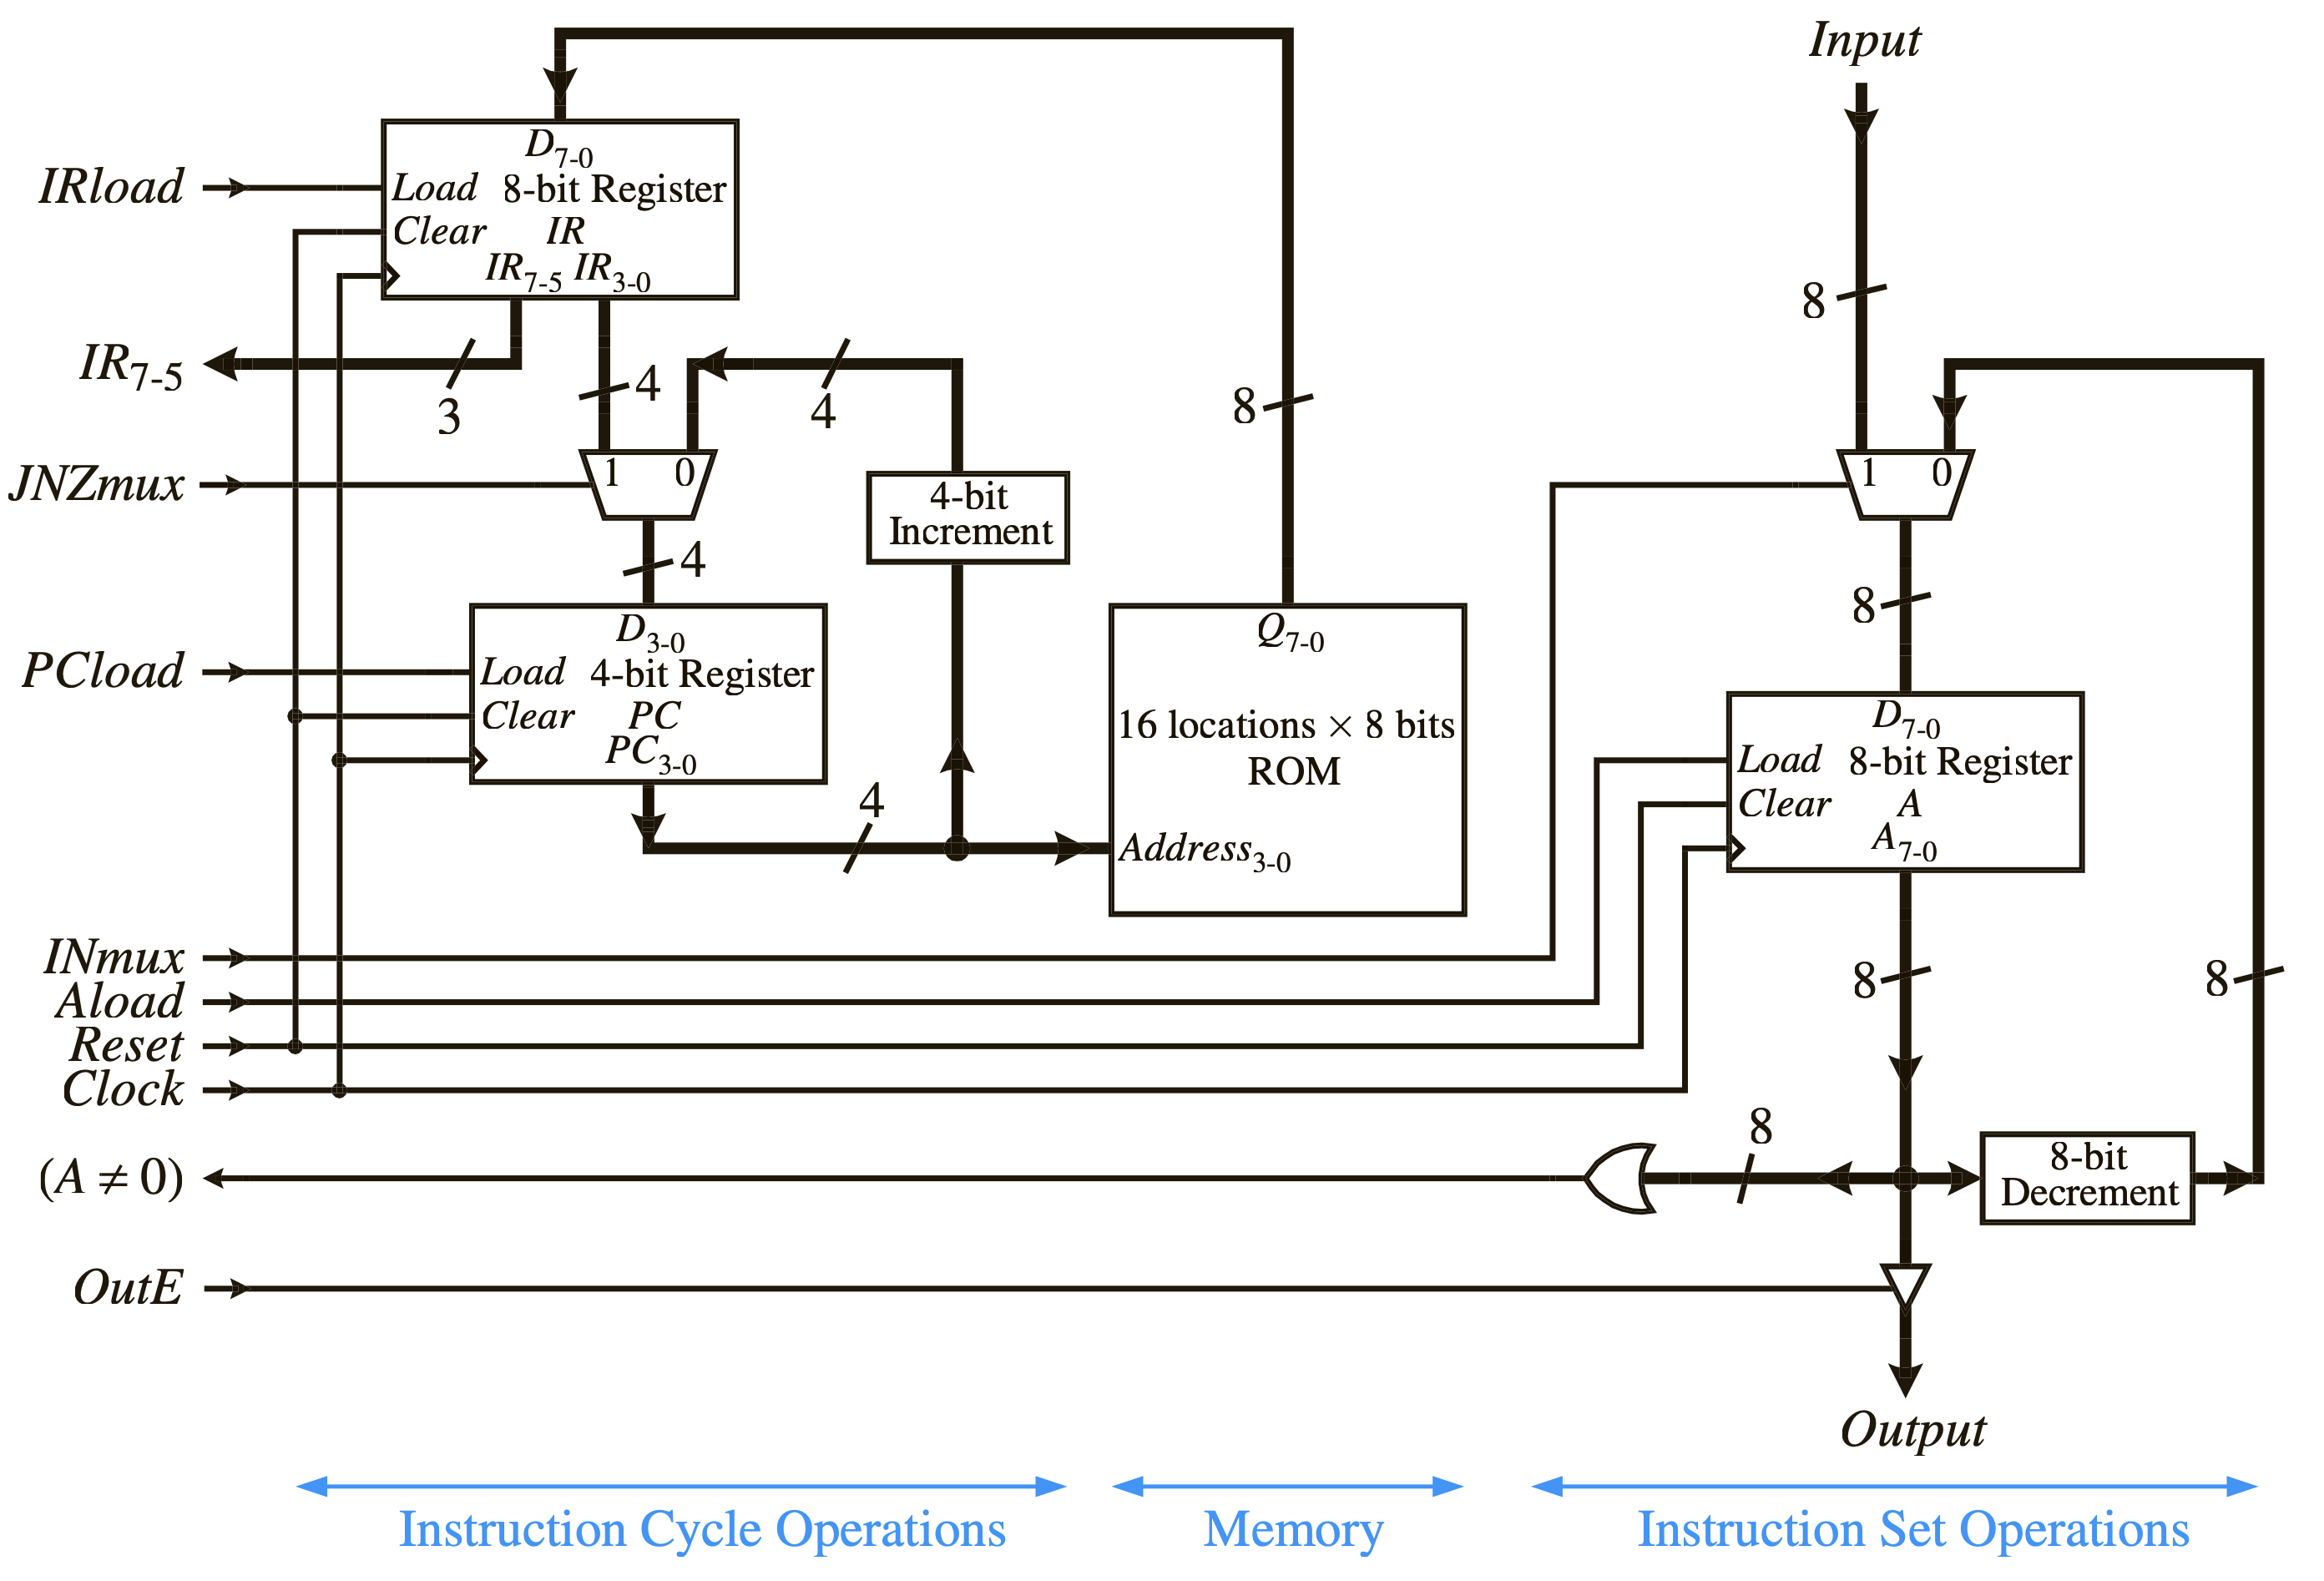
\includegraphics[width=\textwidth]{../assets/lect_10_ec1_datapath.png}
\caption{EC-1 datapath (Lecture 10, Figure 10-1). Left: Instruction Cycle Operations
(\texttt{IR}, \texttt{JNZmux}, \texttt{PC}, the 4-bit Incrementer). Centre: the
16$\times$8 program \textbf{ROM}, addressed \emph{directly} by \texttt{PC} -- there
is no separate address register. Right: Instruction Set Operations (\texttt{INmux},
the Accumulator \texttt{A}, the 8-bit Decrementer, the zero-check producing
$(A \neq 0)$, and the tri-state output buffer gated by \texttt{OutE}).}
\label{fig:datapath-concept}
\end{figure}

Figure~\ref{fig:datapath} is the reference Logisim-Evolution circuit -- build
\emph{exactly this}, component for component, using the same signal names.

\begin{figure}[htbp]
\centering
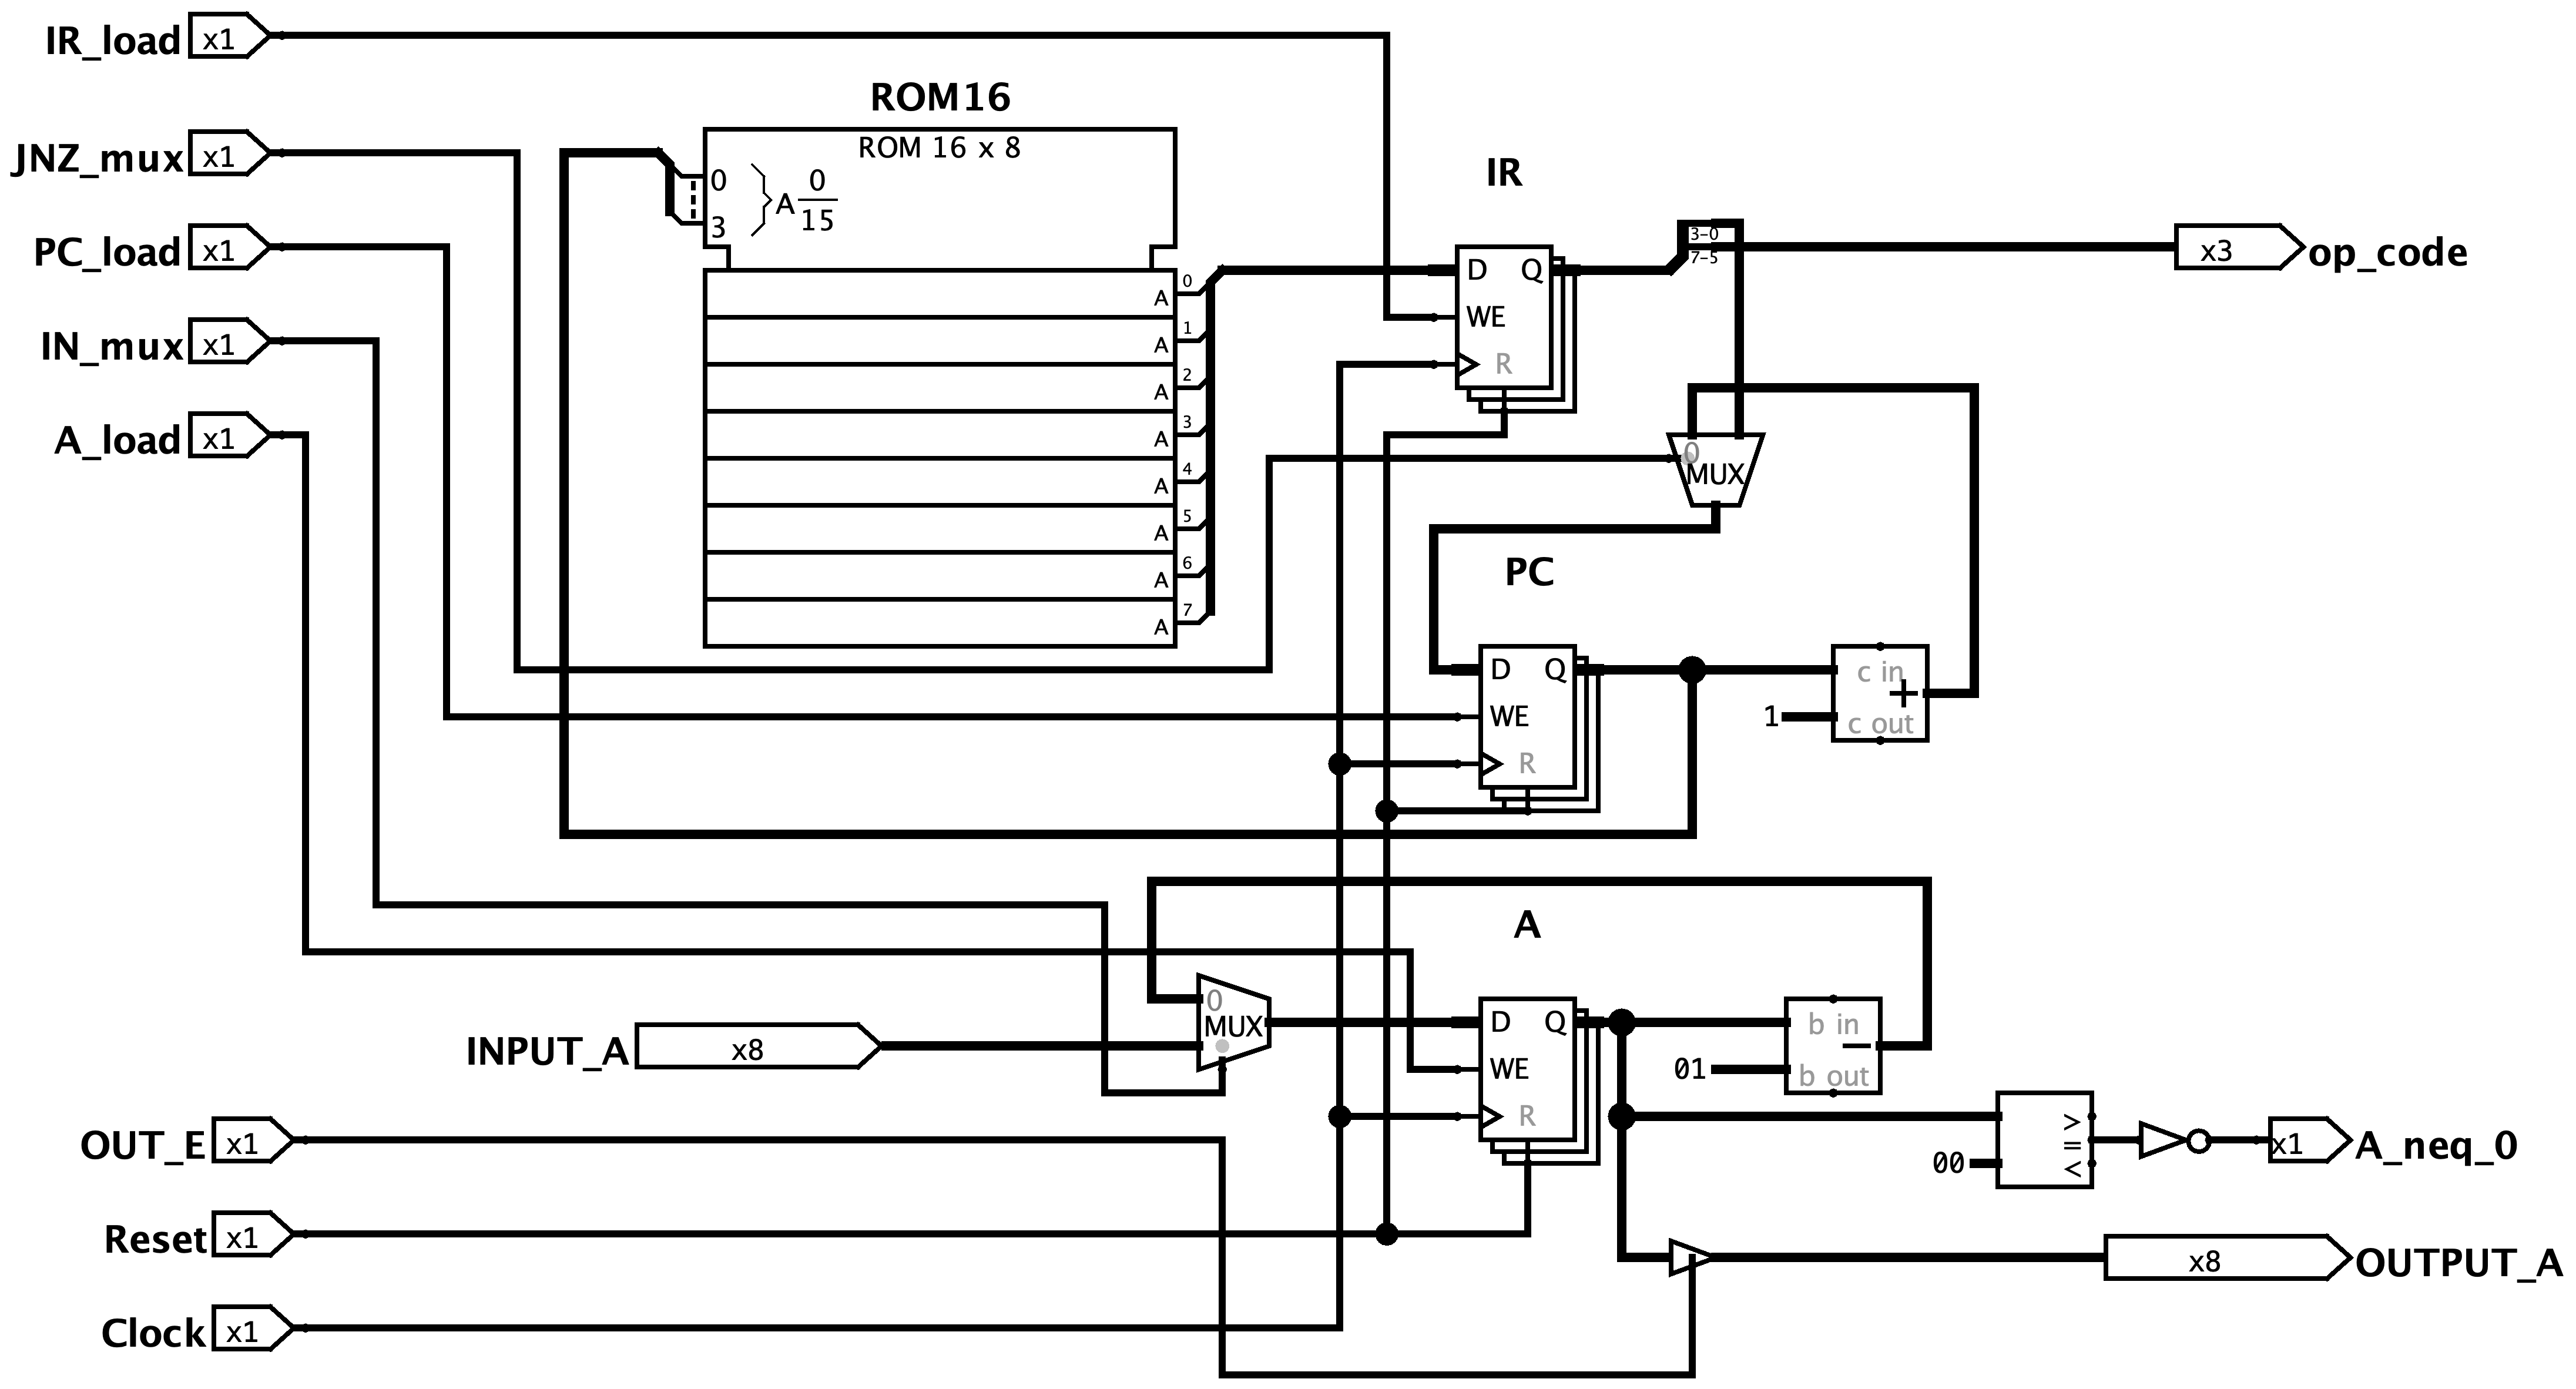
\includegraphics[width=\textwidth]{../assets/ec1_datapath.png}
\caption{Reference \texttt{ec1\_datapath} circuit. \texttt{IR} is loaded from
\texttt{ROM16} (addressed by \texttt{PC}) and split into \texttt{op\_code} (3 bits)
and the jump address; \texttt{JNZ\_mux} selects between \texttt{PC}'s own
\texttt{+1} incrementer and that jump address for \texttt{PC}'s \texttt{D} input.
\texttt{IN\_mux} selects between \texttt{INPUT\_A} and the decrementer's output for
\texttt{A}'s \texttt{D} input; a comparator against \texttt{0} produces
\texttt{A\_neq\_0}, and a tri-state buffer gated by \texttt{OUT\_E} drives
\texttt{OUTPUT\_A}.}
\label{fig:datapath}
\end{figure}

\begin{center}
\begin{tabular}{@{}p{2.9cm}p{9.5cm}@{}}
\toprule
\textbf{Block} & \textbf{Purpose} \\
\midrule
PC & 4-bit register. \texttt{D} comes from \texttt{JNZmux}: input \texttt{0} is
$PC+1$ (Incrementer), input \texttt{1} is \texttt{IR[3:0]} (jump target). Loads
when \texttt{PCload} is asserted. Its output is ROM's \emph{only} address input. \\
IR & 8-bit register, loaded from ROM's data output when \texttt{IRload} is
asserted. \texttt{IR[7:5]} (opcode) goes to the Control Unit; \texttt{IR[3:0]}
goes to \texttt{JNZmux} input \texttt{1}. \\
ROM & 16 $\times$ 8-bit program memory, addressed directly by \texttt{PC}. \\
A (Accumulator) & 8-bit register. \texttt{D} comes from \texttt{INmux}: input
\texttt{1} is the external \texttt{Input} port, input \texttt{0} is the 8-bit
Decrementer's output ($A-1$). Loads when \texttt{Aload} is asserted. \\
Zero check & An 8-input OR (or NOR, inverted) over \texttt{A}, producing
$(A \neq 0)$ for the Control Unit's \texttt{JNZ} test. \\
Tri-state buffer & Drives \texttt{A} onto \texttt{Output} only when \texttt{OutE}
is asserted; high-impedance otherwise. \\
\bottomrule
\end{tabular}
\end{center}

\subsection*{Quick Experiments (Try It)}

\begin{tryit}{PC counts on its own}
Build just the 4-bit \texttt{PC} register, the 4-bit Incrementer, and the
\texttt{JNZmux} (tie its select to \texttt{0} for now). Single-step a manual clock.
\begin{enumerate}[nosep,leftmargin=*]
  \item Does \texttt{PC} count $0,1,2,\ldots,15,0,\ldots$ on its own?
  \item Set \texttt{JNZmux}'s select to \texttt{1} and poke \texttt{IR[3:0]} to some
        value. What happens to \texttt{PC} on the next clock edge?
\end{enumerate}
\end{tryit}

\begin{tryit}{Decrementer wrap-around}
Build the 8-bit Decrementer alone (an 8-bit Adder/Subtractor computing $A-1$) and
poke a few input values with the Poke tool.
\begin{enumerate}[nosep,leftmargin=*]
  \item What does it output for input \texttt{1}? For input \texttt{0}?
  \item In the actual countdown program, \texttt{JNZ} exits the loop the instant
        $A=0$ -- so this wrap-around case never executes. What \emph{would} happen
        if a program kept calling \texttt{DEC} after $A$ reached \texttt{0}?
\end{enumerate}
\end{tryit}

\begin{tryit}{A trivial ROM image}
Build just \texttt{PC} $\to$ \texttt{ROM} $\to$ \texttt{IR} (no Accumulator side
yet). Load this image (a \texttt{HALT} at address \texttt{0}, zeros elsewhere)
with \emph{Load Image}:
\begin{lstlisting}
v2.0 raw
e0
\end{lstlisting}
\begin{enumerate}[nosep,leftmargin=*]
  \item Single-step once. Does \texttt{IR} read \texttt{E0}?
  \item Does \texttt{PC} still advance to \texttt{1} even though the instruction is
        \texttt{HALT}? (Whether the machine actually \emph{stops} is a Control Unit
        job, not a datapath job -- you haven't built that yet.)
\end{enumerate}
\end{tryit}

\section*{In-Lab Exercises (target: 3 hours)}

\begin{labexercise}{PC side \hfill {\small \itshape (25 min)}}
Build the 4-bit \texttt{PC} register, the 4-bit Incrementer, and the
\texttt{JNZmux} (2:1, 4-bit) from Try It 1. Wire \texttt{PC}'s output directly to
where ROM's address input will go -- there is no separate address register
anywhere in this machine.
\end{labexercise}

\begin{labexercise}{Instruction Register \hfill {\small \itshape (15 min)}}
Build the 8-bit \texttt{IR} register. Split its output into \texttt{IR[7:5]}
(opcode, 3 bits) and \texttt{IR[3:0]} (address, 4 bits) using Logisim's Splitter.
\end{labexercise}

\begin{labexercise}{ROM \hfill {\small \itshape (15 min)}}
Add a 16 $\times$ 8-bit \textbf{ROM} component and wire it into the PC/IR pair from
Exercises 1--2: address from \texttt{PC}, data output to \texttt{IR}. Leave it
empty for now -- you will load the countdown program in Exercise 7.
\end{labexercise}

\begin{labexercise}{Accumulator side \hfill {\small \itshape (30 min)}}
Build the 8-bit \texttt{A} register, the 8-bit Decrementer from Try It 2, the
\texttt{INmux} (2:1, 8-bit), the Zero-check (an 8-input OR gate; its output
\emph{is} $(A \neq 0)$ directly), and a Tri-state Buffer on \texttt{A}'s output,
enabled by \texttt{OutE}.
\end{labexercise}

\begin{labexercise}{Design the Control Unit \hfill {\small \itshape (40 min)}}
Using the ISA and the fetch/decode/execute cycle, design the FSM yourself:
\begin{enumerate}[nosep,leftmargin=*]
  \item List every state you need. Start with \texttt{FETCH} and \texttt{DECODE};
        then decide, for each of the 5 instructions, whether it needs a state of
        its own. Do the 3 unused opcodes need one?
  \item Draw the state diagram: a circle per state, an arrow per transition,
        labelled with the opcode (or condition) that causes it. Pay attention to
        \texttt{JNZ} -- how many different next-states can it lead to?
  \item Encode your states in a 3-bit register $Q_2Q_1Q_0$. (Hint: if
        \texttt{DECODE} can transition straight to a state numerically equal to
        the opcode, your next-state logic gets much smaller.)
  \item Derive Boolean equations for $D_2, D_1, D_0$ (next state) and for every
        output (\texttt{IRload}, \texttt{PCload}, \texttt{INmux}, \texttt{Aload},
        \texttt{JNZmux}, \texttt{OutE}, \texttt{Halt}).
\end{enumerate}
Keep this design on paper -- you will check it against Appendix~A and then build it
in Exercise 6.
\end{labexercise}

\begin{labexercise}{Build the Control Unit \hfill {\small \itshape (35 min)}}
Build the 3-bit state register (three D flip-flops, or a Logisim Register), the
state-decoder gates, and the next-state/output logic directly from \emph{your}
Exercise 5 design. Wire $(A\neq0)$ in from the Accumulator side and
\texttt{IR[7:5]} in from \texttt{IR}. Check your design against Appendix~A before
you wire it up if you want a sanity check -- Figure~\ref{fig:control} there shows
a reference circuit, but only look \emph{after} you've built your own.
\end{labexercise}

Figure~\ref{fig:micro} shows how Exercises 1--6 combine into the top-level
\texttt{ec1\_micro} circuit for Exercise 7: \texttt{ec1\_datapath} and
\texttt{ec1\_control} as two subcircuits, with \texttt{Reset} and \texttt{Clock}
fanning out to both, \texttt{INPUT\_A} entering the datapath, \texttt{OUTPUT\_A}
driving a hex display, and \texttt{HALT} driving an LED.

\begin{figure}[htbp]
\centering
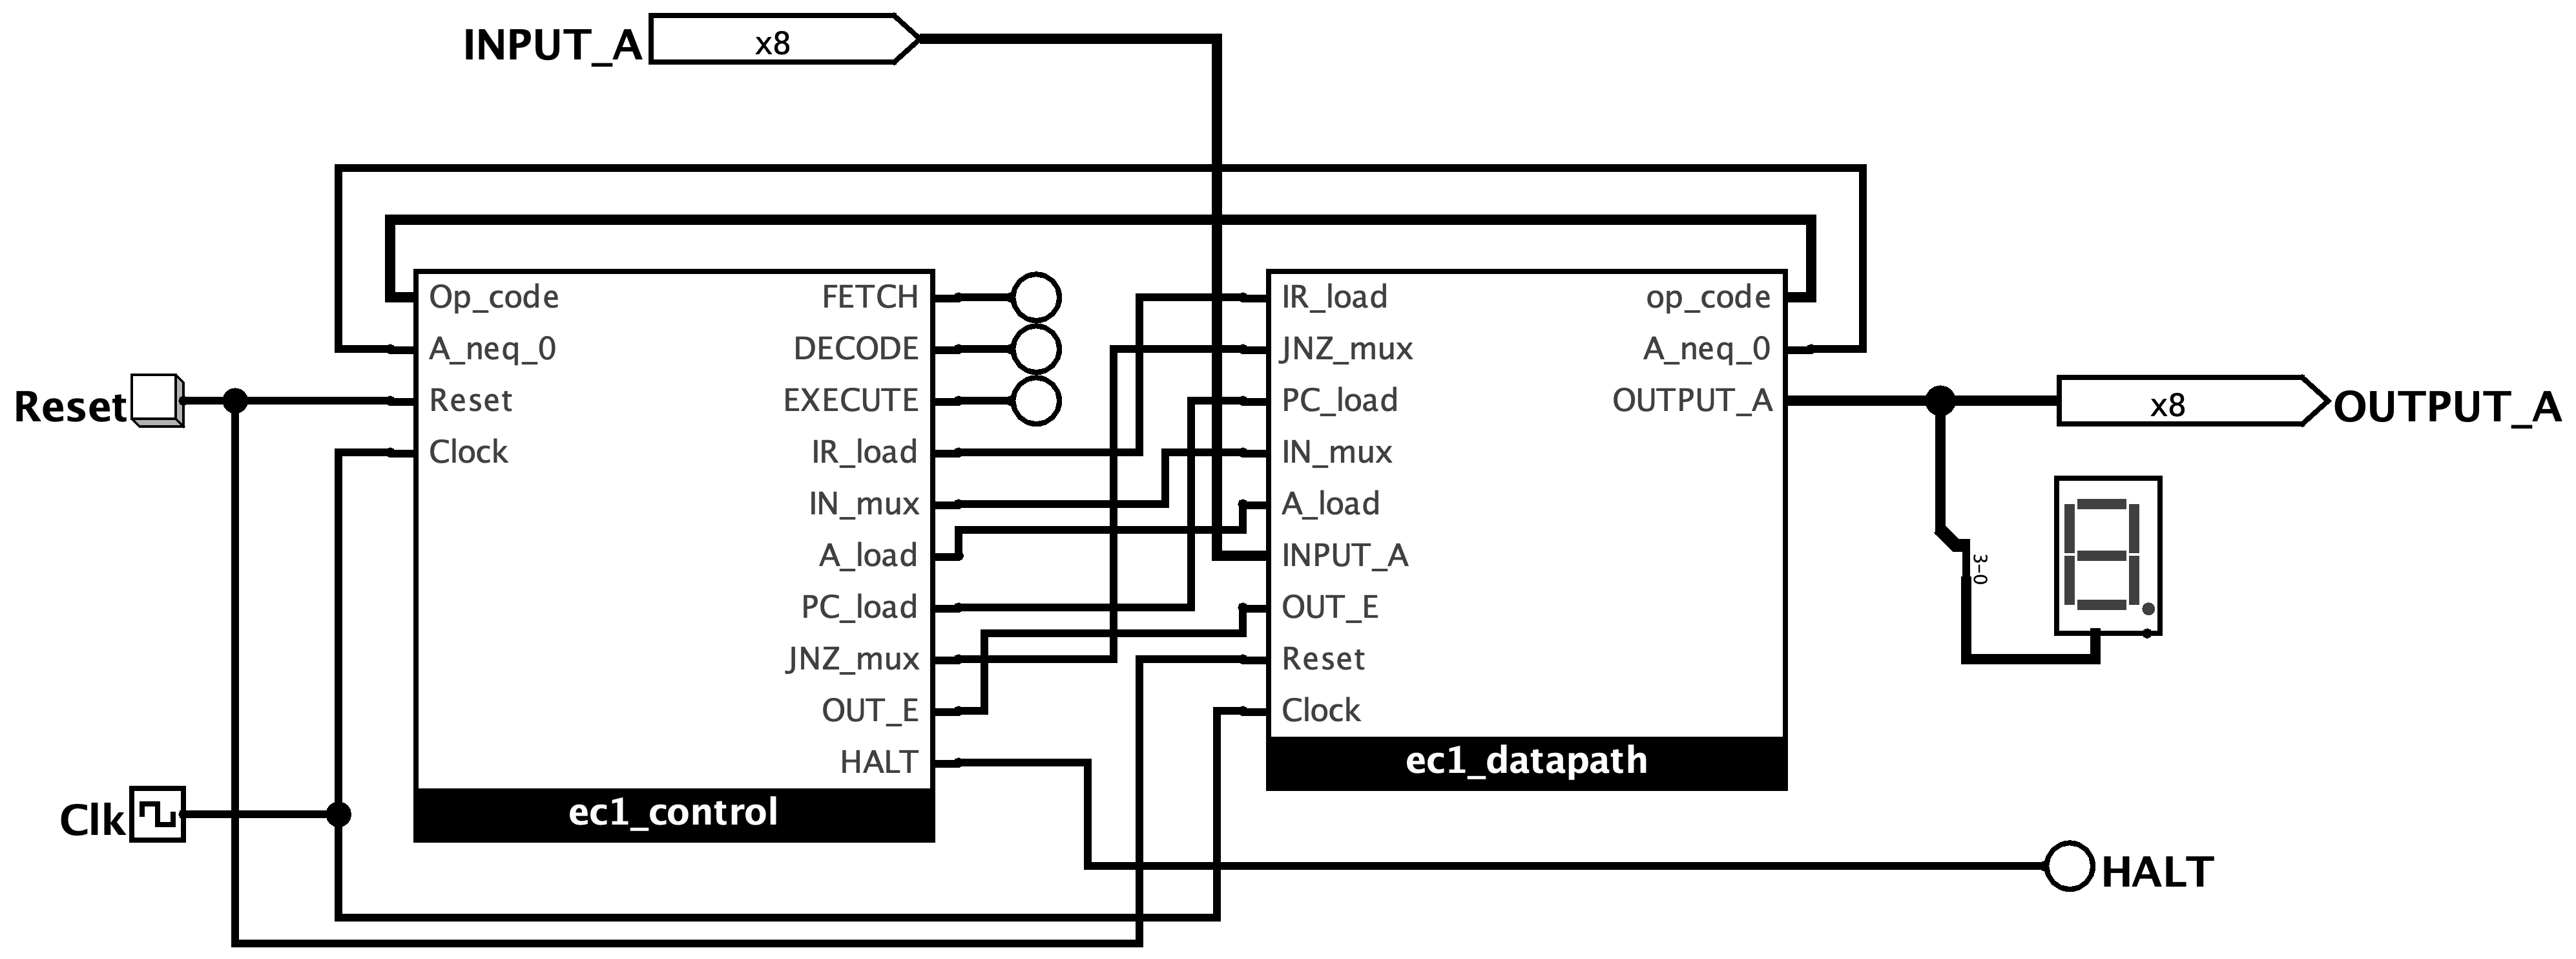
\includegraphics[width=\textwidth]{../assets/ec1_micro.png}
\caption{Reference \texttt{ec1\_micro} top-level circuit: \texttt{ec1\_control} and
\texttt{ec1\_datapath} wired together with \texttt{Reset}, \texttt{Clock},
\texttt{INPUT\_A}, \texttt{OUTPUT\_A} (with hex display), and \texttt{HALT}.}
\label{fig:micro}
\end{figure}

\begin{labexercise}{Assemble, load, and run \hfill {\small \itshape (20 min)}}
Wire Exercises 1--6 together following Figures~\ref{fig:datapath} and
\ref{fig:micro}. Hand-assemble the countdown program below and load it with
ROM's \emph{Load Image}:
\begin{lstlisting}
Addr  Hex  Assembly
00    60   IN A      ; Input to A
01    80   OUT A     ; Output A
02    A0   DEC A     ; Decrement A
03    C1   JNZ 01    ; Jump to 01 if A != 0
04    E0   HALT      ; Halt execution
05-0F 00   (unused)
\end{lstlisting}
Logisim plain-text image (paste into ROM's \emph{Edit Contents}, or save as
\texttt{.txt} and \emph{Load Image}):
\begin{lstlisting}
v2.0 raw
60 80 a0 c1 e0 00 00 00 00 00 00 00 00 00 00 00
\end{lstlisting}
Set \texttt{Input} to \texttt{10} (\texttt{0A} hex) with the Poke tool, then
single-step and confirm \texttt{Output} shows \texttt{10, 9, 8, \ldots, 1} in
turn, followed by \texttt{Halt} going high with the state register no longer
changing.
\end{labexercise}

\begin{aicollab}
\textbf{Try these prompts with an AI tool:}
\begin{itemize}[leftmargin=*,nosep]
  \item ``What is the difference between a hardwired control unit and a
        microprogrammed one?''
  \item ``Given this state transition table [paste yours], derive minimal
        sum-of-products equations for the next-state logic.''
  \item ``Which Logisim-Evolution component should I use for an 8-input OR
        reduction, and how do I wire an 8-bit bus into it?''
\end{itemize}

\medskip\textbf{Critical check -- verify, don't just accept:}
Ask the AI to derive \texttt{PCload} and \texttt{Aload} from your state table.
Then check \emph{every} row of your table against its equations by hand -- not
just the common states, but \texttt{JNZ} specifically, since its conditional term
is the easiest place for a minimization mistake to hide.

\medskip\textbf{Know the limit:}
AI tools will confidently produce next-state equations that satisfy \emph{most}
rows of a state table while silently getting one edge case wrong. It will not
necessarily flag which row it's least sure about -- that's your job.
\end{aicollab}

\takehomebanner

\begin{trace}[The first six clock cycles]
Assume ROM holds the countdown program from Exercise 7 and \texttt{Input} was
poked to \texttt{3} before the first \texttt{FETCH}. Fill in a table with columns
\emph{Cycle, State, PC, IR (hex), A} for the first six clock edges. At which cycle
does \texttt{Output} first show a value, and what is it?
\end{trace}

\begin{bug}[A one-line control equation]
A student built \texttt{PCload = Fetch} (forgetting the \texttt{JNZ} term
entirely) but wired everything else correctly. Predict exactly what the
countdown program's \texttt{Output} sequence looks like when run on this
machine, and explain why it goes wrong where it does.
\end{bug}

\begin{writecode}[Design a sixth instruction]
EC-1 has three unused opcodes. Using \texttt{010}, design \texttt{INC A}
($A \leftarrow A+1$). Write its encoding, describe any new datapath component or
mux input it needs (if any), and write the modified \texttt{Aload} and
\texttt{INmux} equations (or a new control signal) required to support it.
\end{writecode}

\begin{drawex}{Extended state diagram}
Redraw your Exercise 5 state diagram with \texttt{INC} (from the previous
exercise) added as an eighth state. Label its transition from \texttt{DECODE}
and its return to \texttt{FETCH}. Compare against your original diagram: how many
new states, gates, and wires did one extra instruction actually cost?
\end{drawex}

\section*{Reflection}

In one short paragraph, compare EC-1's control unit to Lab 1's control-word
machine. Both machines execute a sequence of ``instructions'' stored in ROM and
both can jump conditionally -- but EC-1 has an Instruction Register, an opcode
field, and a multi-state hardwired FSM, while Lab 1's machine has neither. What
did EC-1's FSM \emph{buy} you that Lab 1's machine does not have? What did Lab
1's machine give up to avoid needing one?

\newpage
\section*{Appendix A: Reference Control-Unit Design (Self-Check)}

Use this \emph{after} attempting Exercise 5 -- not before.

\begin{center}
\begin{tabular}{@{}clp{7.6cm}@{}}
\toprule
$Q_2Q_1Q_0$ & \textbf{State} & \textbf{What happens} \\
\midrule
000 & FETCH  & $IR \leftarrow \text{ROM}[PC]$, $PC \leftarrow PC+1$. \\
001 & DECODE & Inspect \texttt{IR[7:5]}; no datapath signals asserted. \\
011 & INPUT  & $A \leftarrow \text{Input}$. \\
100 & OUTPUT & $\text{Output} \leftarrow A$. \\
101 & DEC    & $A \leftarrow A - 1$. \\
110 & JNZ    & If $A \neq 0$: $PC \leftarrow IR[3:0]$; either way, return to \texttt{FETCH}. \\
111 & HALT   & Stop (self-loop). \\
\bottomrule
\end{tabular}
\end{center}

\begin{figure}[h!]
\centering
\begin{tikzpicture}[
    ->, >=stealth, auto, node distance=2.1cm, scale=0.8, every node/.append style={scale=0.8},
    every state/.style={thick, fill=accentlight, minimum size=1.2cm},
    initial text=$ $
]
    \node[state, initial] (FETCH) {FETCH};
    \node[state, below of=FETCH, node distance=2.3cm] (DECODE) {DECODE};
    \node[state, below of=DECODE, node distance=3cm] (DEC) {DEC};
    \node[state, left of=DEC, node distance=2.6cm] (OUTPUT) {OUTPUT};
    \node[state, left of=OUTPUT, node distance=2.6cm] (INPUT) {INPUT};
    \node[state, right of=DEC, node distance=2.6cm] (JNZ) {JNZ};
    \node[state, right of=JNZ, node distance=2.6cm] (HALT) {HALT};

    \path (FETCH) edge node {} (DECODE);

    \path (DECODE) edge node [above, sloped, near end] {Op=011} (INPUT)
          (DECODE) edge node [above, sloped, near end] {Op=100} (OUTPUT)
          (DECODE) edge node {Op=101} (DEC)
          (DECODE) edge node [above, sloped, near end] {Op=110} (JNZ)
          (DECODE) edge node [above, sloped, near end] {Op=111} (HALT);

    \path (DECODE) edge [bend left=30, align=center] node [left] {Op=00x} (FETCH);

    \path (INPUT)  edge [bend left=45] node {} (FETCH)
          (OUTPUT) edge [bend left=45] node {} (FETCH)
          (DEC)    edge [bend right=45]  node {} (FETCH)
          (JNZ)    edge [bend right=45] node {} (FETCH);

    \path (HALT)   edge [loop right] node {} (HALT);
\end{tikzpicture}
\caption{EC-1 Control Unit FSM (Lecture 10, Figure 10-3).}
\end{figure}

Using $\text{Fetch}=\bar Q_2\bar Q_1\bar Q_0$, $\text{Decode}=\bar Q_2\bar Q_1 Q_0$,
$\text{Input}=\bar Q_2 Q_1 Q_0$, $\text{Output}=Q_2\bar Q_1\bar Q_0$,
$\text{Dec}=Q_2\bar Q_1 Q_0$, $\text{JNZ}=Q_2 Q_1 \bar Q_0$,
$\text{Halt}=Q_2Q_1Q_0$, and $O_2O_1O_0=\texttt{IR[7:5]}$:

\begin{center}
\begin{tabular}{@{}ll@{}}
\toprule
\textbf{Next state} & \textbf{Equation} \\
\midrule
$D_2$ & $= \text{Decode}\cdot O_2 + \text{Halt}$ \\
$D_1$ & $= \text{Decode}\cdot O_1\cdot(O_2+O_0) + \text{Halt}$ \\
$D_0$ & $= \text{Fetch} + \text{Decode}\cdot O_0\cdot(O_2+O_1) + \text{Halt}$ \\
\bottomrule
\end{tabular}
\hspace{1cm}
\begin{tabular}{@{}ll@{}}
\toprule
\textbf{Output} & \textbf{Equation} \\
\midrule
\texttt{IRload} & $= \text{Fetch}$ \\
\texttt{PCload} & $= \text{Fetch} + \text{JNZ}\cdot(A \neq 0)$ \\
\texttt{INmux}  & $= \text{Input}$ \\
\texttt{Aload}  & $= \text{Input} + \text{Dec}$ \\
\texttt{JNZmux} & $= \text{JNZ}$ \\
\texttt{OutE}   & $= \text{Output}$ \\
\texttt{Halt}   & $= \text{Halt}$ \\
\bottomrule
\end{tabular}
\end{center}

Figure~\ref{fig:control} is a reference \texttt{ec1\_control} circuit implementing
the design above -- one way to build it, not the only way. Compare it against your
own next-state and output equations only \emph{after} you've derived them yourself.

\begin{figure}[htbp]
\centering
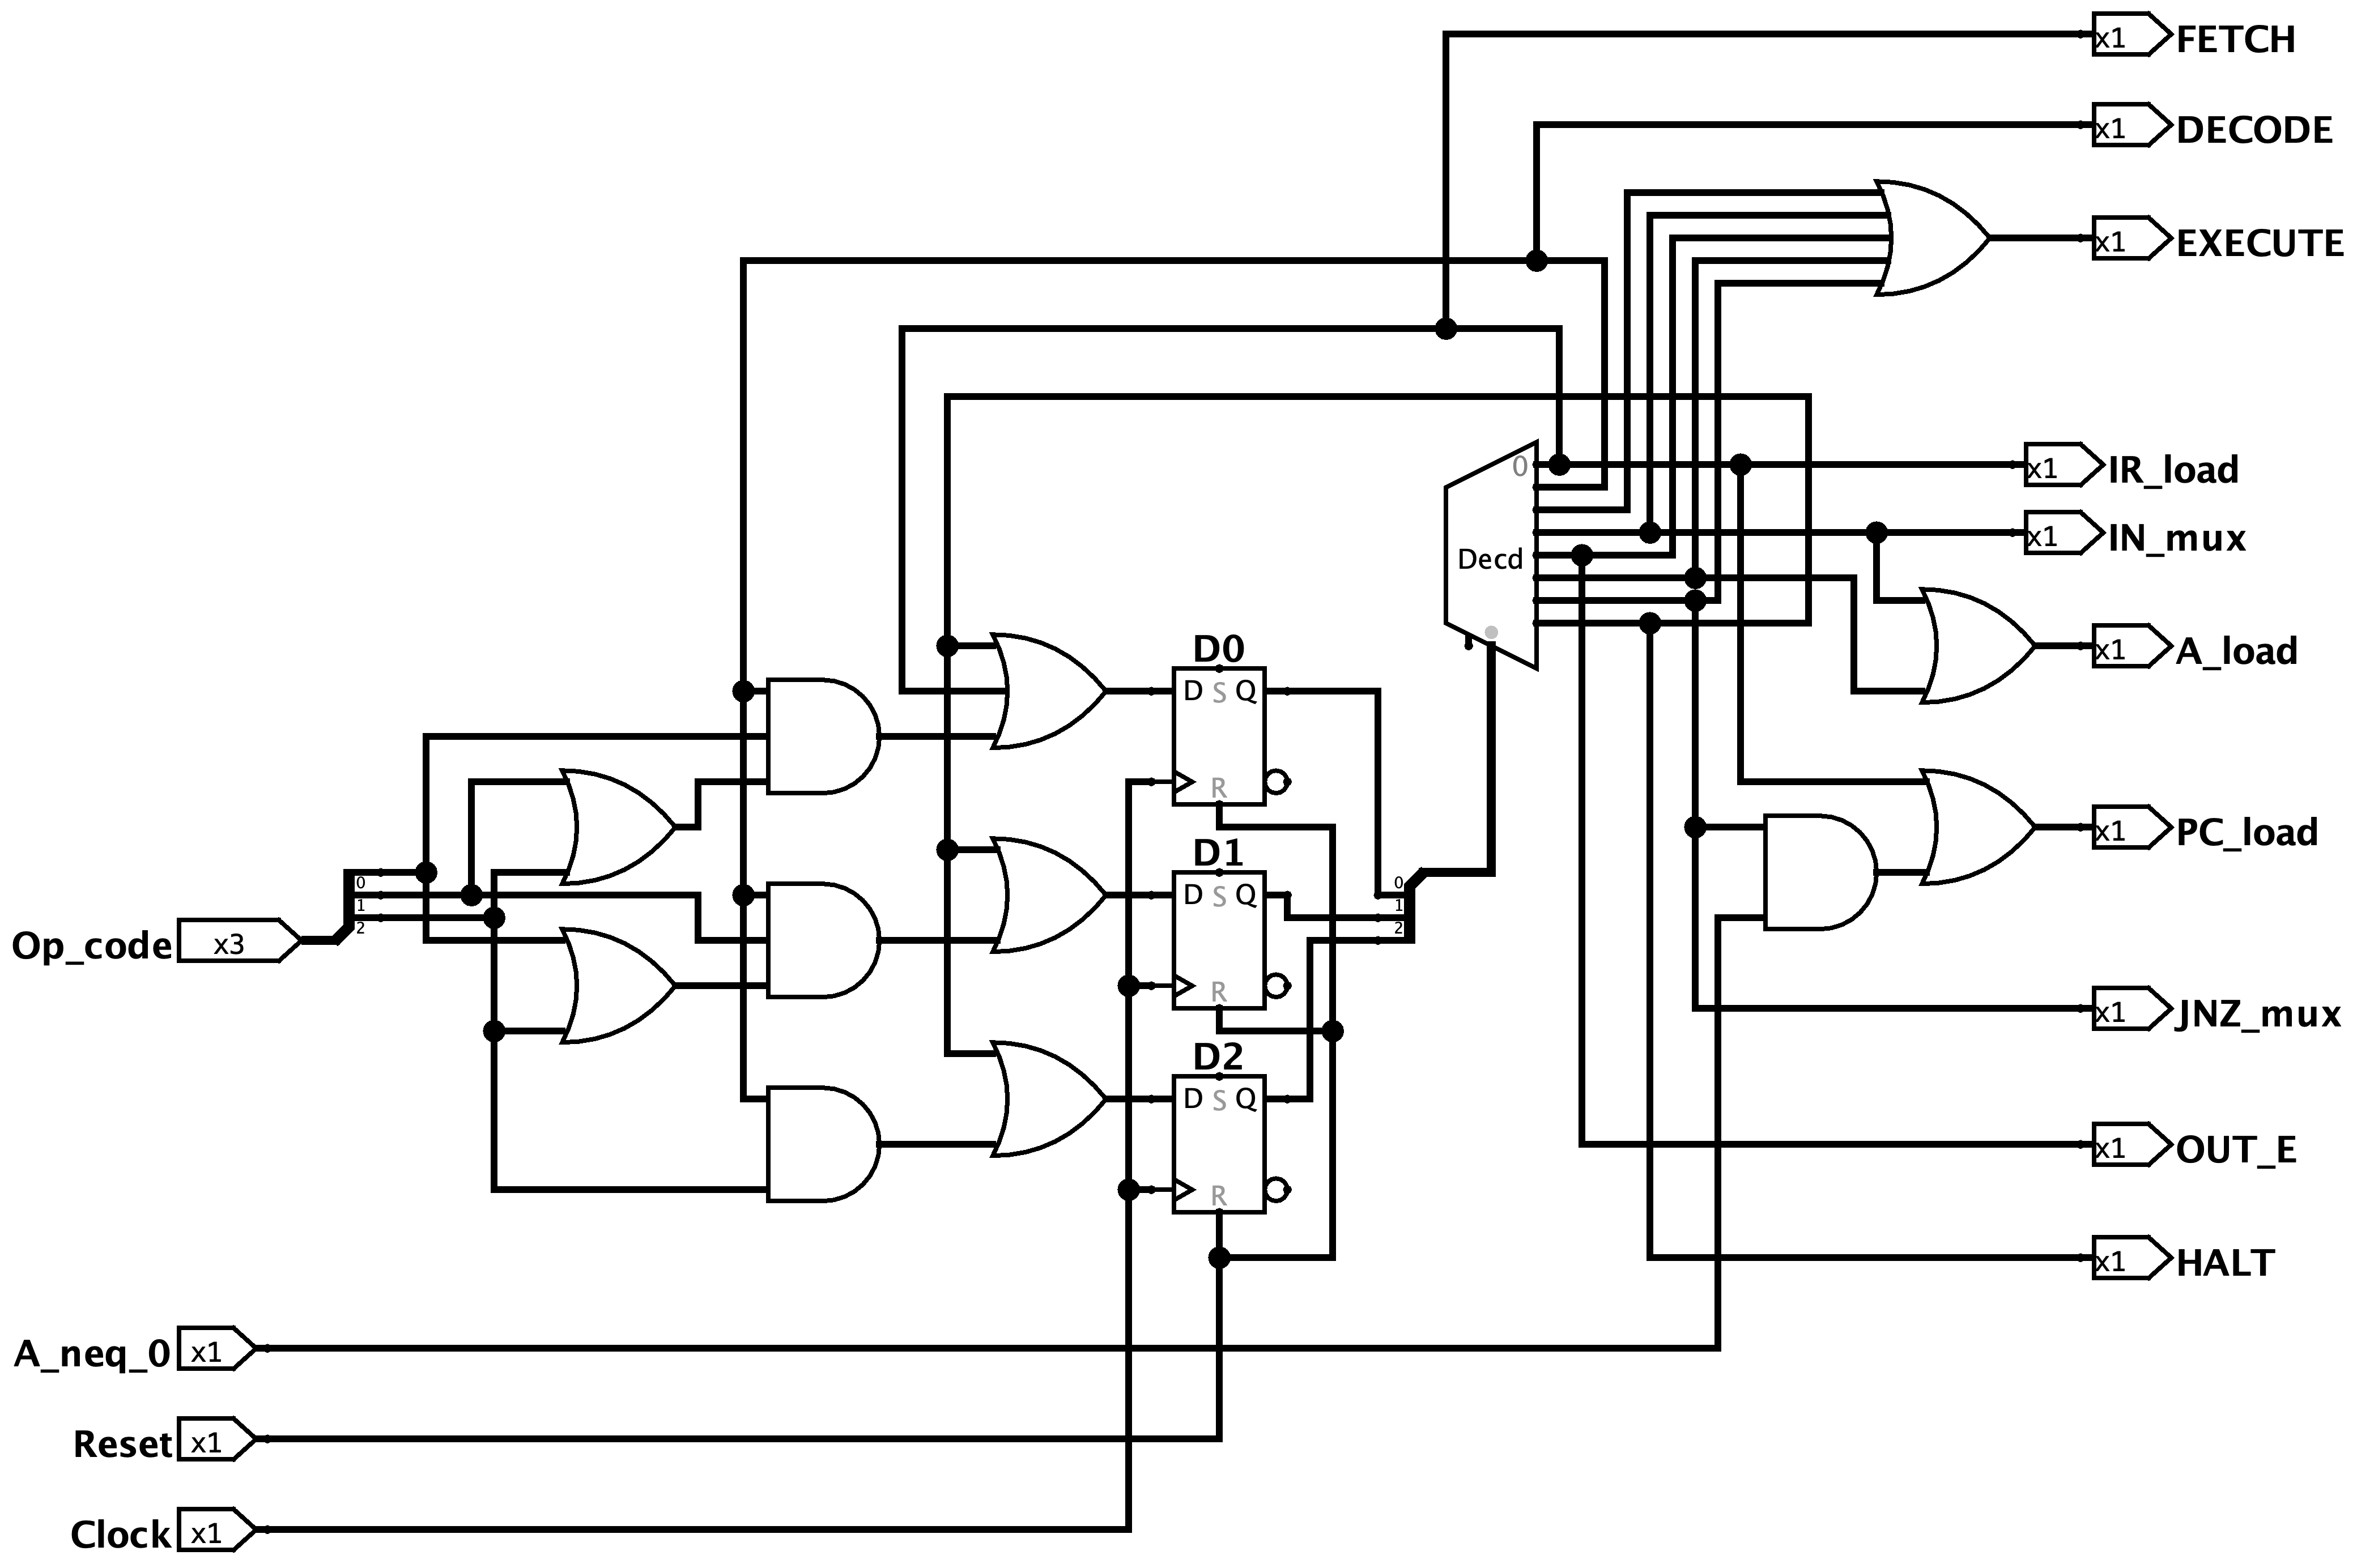
\includegraphics[width=\textwidth]{../assets/ec1_control.png}
\caption{Reference \texttt{ec1\_control} circuit. \texttt{Op\_code} feeds the
next-state logic for the \texttt{D0}, \texttt{D1}, \texttt{D2} state flip-flops
(with \texttt{Reset} and \texttt{Clock}); the resulting 3-bit state, together with
$(A\neq0)$, drives a decoder/mux (\texttt{Decd}) that asserts \texttt{IR\_load},
\texttt{IN\_mux}, \texttt{A\_load}, \texttt{PC\_load}, \texttt{JNZ\_mux},
\texttt{OUT\_E}, and \texttt{HALT} in the correct states, plus the
\texttt{FETCH}/\texttt{DECODE}/\texttt{EXECUTE} status LEDs.}
\label{fig:control}
\end{figure}

\end{document}
